
\section{Conclusion}
\subsection{Summary}
\begin{frame}{Class Summary}{Graph Basics}
  \begin{itemize}
    \item Graph Problems come in a large variety of types;
    \item But Many Algorithms are variations on BFS and DFS;
    \begin{itemize}
      \item Connected Components and Flood Fill;
      \item Topological Sort;
      \item Articulation Points and Bridges;
      \item Minimum Spanning Trees;
    \end{itemize}
    \item There are several special cases for graph problems:
  \end{itemize}

  \begin{block}{Some common special cases}
    \begin{itemize}
    \item Graphs with 0 or 1 Vertices; Graphs with 0 nodes;
    \item Unconnected Graphs;
    \item Self loops;
    \item Double edges;
    \end{itemize}
  \end{block}
\end{frame}

\begin{frame}{Class Summary}{Theme for Next Week}

  Graph Path Search and Weighted Graphs:
  \begin{itemize}
    \item Shortest Paths (Single Source and All Pairs);
    \item Network Flow;
    \item Graph Matching;
  \end{itemize}\bigskip

  \begin{block}{Graph Code Library}
    Graph problems share a lot of common code. I recommend that you prepare a code library as you learn new algorithms.
    \bigskip
    \begin{itemize}
    \item Visited node flags and adjacency lists;
    \item Parent and children lists;
    \item Different algorithms;
    \item etc;
    \end{itemize}
  \end{block}
\end{frame}

\subsection{Homework Discussion}

\begin{frame}{This Week's Problems}
  \begin{itemize}
  \item Dominator -- Discussed in class;
  \item Forwarding Emails
  \item Ordering
  \item Place the Guards
  \item Doves and Bombs
  \item Come and Go
  \item ACM Contest and Blackout
  \item Ancient Messages
  \end{itemize}
\end{frame}


\begin{frame}{Problem Hints}{Forwarding E-mails}
  \begin{block}{Problem Summary}
    \begin{itemize}
      \item In a list of $N$ people, every person $i$ forwards e-mails to a single person $j$.
      \item If you want to form the longest e-mail chain, where do you start?
      \item {\bf Output:} The person $k$ that starts the longest chain;
    \end{itemize}
  \end{block}\bigskip

  \begin{itemize}
    \item The time limit is not very large, you should find an $O(n)$ solution;
    \medskip

    \item How do you deal with loops?
  \end{itemize}
\end{frame}

\begin{frame}{Problem Hints}{Ordering and Palace Guards}
  \begin{block}{Ordering}
    \begin{itemize}
      \item {\bf Outline:} List all possible orderings of a given Direct Acyclic Graph;
      \item {\bf Hint:} In the lecture, we saw an algorithm for a single ordering -- for this problem, you need to generalize it for all orderings;
    \end{itemize}
  \end{block}

  \begin{block}{Palace Guards}
    You need to find a guard assignment for the city that obey the rules:
    \begin{itemize}
      \item All roads need {\bf one guard}.
      \item No road can have {\bf two guards}.
    \end{itemize}\bigskip

    Note that for some inputs a solution is impossible.
  \end{block}
\end{frame}

\begin{frame}{Problem Hints}{Doves and Bombs / Come and Go}
    \begin{block}{Doves and Bombs}
      \begin{itemize}
        \item {\bf Outline:} You must choose one station (vertex) to remove, so that the number of unconnected subgraphs is maximum;
        \item {\bf Hint:} Do you need to calculate the CCs every time you test a vertex, or is there a better way?
      \end{itemize}
    \end{block}

    \begin{block}{Come and Go}
      \begin{itemize}
        \item {\bf Outline:} For a city road map, you must check if that city is strongly connected (you can go from every node i to every node j) or not;
        \item {\bf Hint:} Can you use the algorithm of strongly connected components for this?
      \end{itemize}
    \end{block}
\end{frame}

\begin{frame}{Problem Hints}{ACM Contest and Blackout}
    \begin{block}{Outline}
      Given a graph of a powerplant and several schools, you have to find the {\bf two} cheapest graphs that connect all the nodes.\bigskip

      {\bf Output}: Cost of cheapest graph, and cost of 2nd cheapest graph.
    \end{block}\bigskip

    {\bf Hint:} The cheapest graph could be found using the MST algorithm. But how do we find the {\bf second} cheapest graph?
\end{frame}

\begin{frame}{Problem Hints}{Ancient Message}
  \begin{block}{Outline}
    \begin{itemize}
      \item {\bf Input:} A pixel image containing one or more "egyptian letters";
      \item {\bf Output:} Identify which letters appear in the image;
    \end{itemize}
  \end{block}

  {\bf Hints:}
  \begin{itemize}
    \item Note that the input is in hexadecimal format;
    \item First: Think about how to count the number of characters in an image. This will help you think a way to identify the characters.
    \item Pay attention to the "Rules" in the problem description.
  \end{itemize}

  \begin{center}
  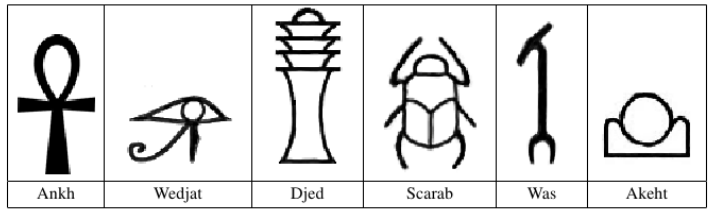
\includegraphics[height=.25\textheight]{img/ancient_messages_letters.png}\hspace{1cm}
  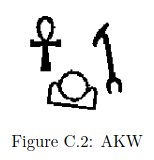
\includegraphics[height=.25\textheight]{img/ancient_messages_example.png}
  \end{center}
\end{frame}
